% --------------------------------------------------------------
% This is all preamble stuff that you don't have to worry about.
% Head down to where it says "Start here"
% --------------------------------------------------------------

\documentclass[12pt]{article}

\usepackage[margin=1in]{geometry}
\usepackage{amsmath,amsthm,amssymb}
\usepackage{graphicx} %This allows to include eps figures

% This is to include code
\usepackage{listings}
\usepackage{xcolor}
\definecolor{dkgreen}{rgb}{0,0.6,0}
\definecolor{gray}{rgb}{0.5,0.5,0.5}
\definecolor{mauve}{rgb}{0.58,0,0.82}
\lstdefinestyle{Python}{
    language        = Python,
    basicstyle      = \ttfamily,
    keywordstyle    = \color{blue},
    keywordstyle    = [2] \color{teal}, % just to check that it works
    stringstyle     = \color{green},
    commentstyle    = \color{red}\ttfamily
}

\newcommand{\N}{\mathbb{N}}
\newcommand{\Z}{\mathbb{Z}}

\newenvironment{theorem}[2][Theorem]{\begin{trivlist}
\item[\hskip \labelsep {\bfseries #1}\hskip \labelsep {\bfseries #2.}]}{\end{trivlist}}
\newenvironment{lemma}[2][Lemma]{\begin{trivlist}
\item[\hskip \labelsep {\bfseries #1}\hskip \labelsep {\bfseries #2.}]}{\end{trivlist}}
\newenvironment{exercise}[2][Exercise]{\begin{trivlist}
\item[\hskip \labelsep {\bfseries #1}\hskip \labelsep {\bfseries #2.}]}{\end{trivlist}}
\newenvironment{reflection}[2][Reflection]{\begin{trivlist}
\item[\hskip \labelsep {\bfseries #1}\hskip \labelsep {\bfseries #2.}]}{\end{trivlist}}
\newenvironment{proposition}[2][Proposition]{\begin{trivlist}
\item[\hskip \labelsep {\bfseries #1}\hskip \labelsep {\bfseries #2.}]}{\end{trivlist}}
\newenvironment{corollary}[2][Corollary]{\begin{trivlist}
\item[\hskip \labelsep {\bfseries #1}\hskip \labelsep {\bfseries #2.}]}{\end{trivlist}}

\begin{document}

% --------------------------------------------------------------
%                         Start here
% --------------------------------------------------------------

%\renewcommand{\qedsymbol}{\filledbox}

\title{Homework 1}%replace X with the appropriate number
\author{Nalet Meinen\\ %replace with your name
Introduction to Signal and Image Processing
}

\maketitle

\section{Regular Tesselation}
\subsection{}
  There are three shapes that satisfy the two conditions above: triangles, squares and regular hexagon.
\subsection{}
\newtheorem{thm}{Theorem}
\begin{thm}
  There are three shapes that satisfy the two conditions above: triangles, squares and regular hexagon.
\end{thm}

\begin{proof}
The sum of the angles in a poligon is $180(a-2)$, a is the number of angles. 
Using the three polygons from above we know that in all three polygons the sum of the angles 
where the vertices meet is $360$, also point $b$. By that circumstances we can use
\[ \frac{180(a-2)}{a}b=360 \]
In a simple matter this leads us to
\[ (a-2)b=2a \]
The result of the equation above leads us to 5 solutions: 
\[ a=-2,b=1;a=1,b=-2,a=3,b=6;a=4,b=4;a=6,b=3 \]
As can only use the positives integer soultions, we have (b corresponds number of edges) the polygons
with 3,4 and 6 edges.
\end{proof}
\newpage

\section{Lloyd-Max quantization}
\subsection{}
Following the notes quanzization from the lecture: We can compute the partial derivatives with respect to $z_{k}$
\[ \delta = \sum_{k=1}^{K} \int_{z_{k}}^{z_{k+1}} (z-q_{k})^2p(z) dz  \]
\[ \frac{\partial \delta}{\partial z_{k}} = (z_{k} - q_{k+1})^2 p(z_{k}) - (z_{k} - q_{k})^2 p(z_{k}) = 0\]
\[ (z_{k} - q_{k+1})^2 p(z_{k}) - (z_{k} - q_{k})^2 p(z_{k}) = 0\]
\[ (z_{k} - q_{k+1})^2 - (z_{k} - q_{k})^2 = 0\]
\[ z_{k}^2 - 2 q_{k+1} z_{k} + q_{k+1}^2 - z_{k}^2 - q_{k}z_{k} + q_{k}^2 = 0\]
\[ 2 z_{k} ( q_{k+1} - q_{k} ) + q_{k+1}^2 + q_{k}^2 = 0\]
\[ 2 z_{k} = \frac{q_{k+1}^2 + q_{k}^2}{q_{k+1} - q_{k}} \implies 2 z_{k} = \frac{q_{k-1}^2 + q_{k}^2}{q_{k-1} + q_{k}} \]
\[ 2 z_{k} = \frac{q_{k-1} + q_{k}}{1} \]
\[ z_{k} = \frac{q_{k-1} + q_{k}}{2} \]
\subsection{}
\[ \delta = \sum_{k=1}^{K} \int_{z_{k}}^{z_{k+1}} (z-q_{k})^2p(z) dz  \]
\[ \frac{\partial \delta}{\partial q_{k}} = \int_{z_{k}}^{z_{k+1}} (z-q_{k})^2p(z) dz = 0\]
\[ \frac{\partial \delta}{\partial q_{k}} \int_{z_{k}}^{z_{k+1}} z^2 p(z) - 2q_{k}z p(z)  + q_{k}^2 p(z) dz = 0\]
\[ \frac{\partial \delta}{\partial q_{k}} (q_{k} \int_{z_{k}}^{z_{k+1}} - 2z p(z) dz + q_{k}^2 \int_{z_{k}}^{z_{k+1}} p(z) dz) = 0\]
\[ \int_{z_{k}}^{z_{k+1}} - 2z p(z) dz + 2q_{k} \int_{z_{k}}^{z_{k+1}} p(z) dz = 0\]
\[ q_{k} = \frac{\int_{z_{k}}^{z_{k+1}} 2z p(z) dz} {2 \int_{z_{k}}^{z_{k+1}} p(z) dz}\]
\[ q_{k} = \frac{\int_{z_{k}}^{z_{k+1}} z p(z) dz}{\int_{z_{k}}^{z_{k+1}} p(z) dz}\]

\subsection{}
lloyd  will give use the converge, but the solution could be a local minimum. The goal is a optimum quantizer, even distributed groups.
Both equations converge in a coordinate descent fashion.

\section{Chamfer distances}
\begin{figure}[!htb]
  \centering
  %omit extension of file. pdflatex will convert to pdf automatically.
  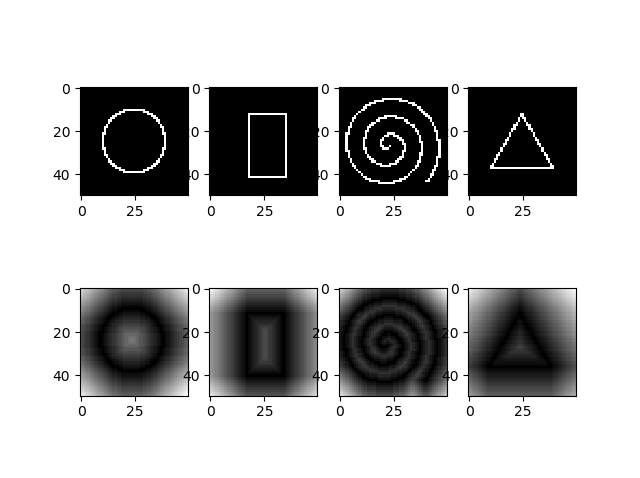
\includegraphics[width=0.8\textwidth]{pics/hw1_ex3_template_chamfer.png}
  \caption{Result of the chamfer distances in given images.}
  \end{figure}
\newpage
\section{Bilinear interpolation}
\begin{figure}[!htb]
  \centering
  %omit extension of file. pdflatex will convert to pdf automatically.
  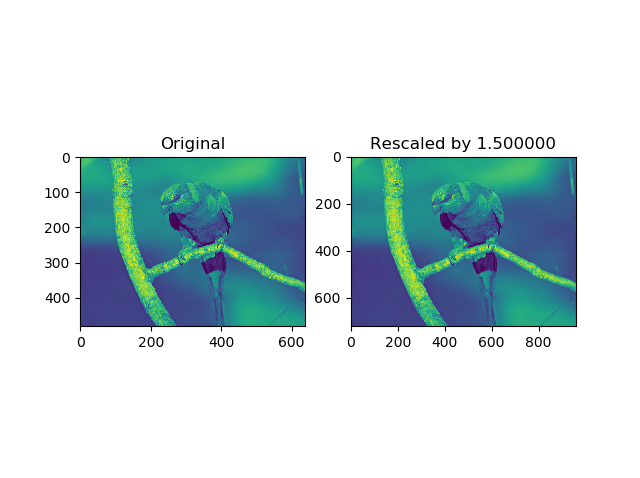
\includegraphics[width=0.8\textwidth]{pics/hw1_ex4_template_bilinear_interp.png}
  \caption{Result of the bilinear interpolation in the image bird.jpg.}
  \end{figure}
\end{document}